\section{Problem Setups}
Due to the inherent limitations of current computing systems, 
obtaining sufficiently precise solutions is both computationally expensive and time-consuming. 
These challenges arise from the constraints imposed by the clock speed of computing units, 
as described by 
Moore's Law \cite{Moore_Law}, 
as well as the relatively low communication speeds between these units. 
While modern numerical methods have advanced to a level where they can produce 
satisfactory results within acceptable time frames across many research domains, 
the increasing scale of problems we aim to solve has driven the search for more 
cost-effective approaches. This has led to a growing interest in neural networks as a promising alternative.

In this project, I aim to evaluate the performance of the Finite-Difference Time-Domain (FDTD) 
method and the Physics-Informed Neural Network (PINN) model within parallelized computing 
environments by find the steady-state solution of PDEs.
These two methodologies broadly represent the current approaches to 
handling PDEs, specifically 
CPU-based parallelization and GPU-based parallelization.

\subsection{General Form}
Starting with the general form of the PDEs, rather than the specific euqations, is because 
different equations give perform differently on the same compute system.
To this end, consider the previously discussed form of PDEs shown in 
equation \ref{EQ_General_PDEs} which parametrized by number $\lambda$ and an operator $\mathcal{N}[\cdot; \lambda]$.
Moreover, we assume the variable $x$ is a 2D or 3D spatio vector which is written in 
$\vec{x} \in \mathbb{R}^d$, $d = 2, 3$.
The domain of this PDE system is considered between $0$ and $1$, where is denoted with $\Omega = [0, 1]^d$, $d = 2,3$.
To these setups, we have the general form of the PDEs we are going to investigated, shown in equations \ref{EQ_General_Form_PDE}
\begin{align}\label{EQ_General_Form_PDE}
  &\frac{\partial u}{\partial t}\left(t,\vec{x}\right) + \mathcal{N}\left[u(t,\vec{x});\lambda\right] = 0, &\vec{x}\in\Omega, &t\in[0, +\infty) \nonumber\\
  &u\left(0,\vec{x}\right) = \varphi (\vec{x}), &\vec{x}\in\Omega & \\
  &u\left(t,\vec{x}\right) = g (t,\vec{x}),     &\vec{x}\in \overline{\Omega}, &t\in[0, +\infty) \nonumber
\end{align}
The boundary condition shown in E.q. \ref{EQ_General_Form_PDE} is Dirichlet Condition known as first type boundary condition, where as the 
second type boundary condition (Von Neumman) [E.q. \ref{EQ_Von_Neumman_BC}] gives the other form of $u(t,\vec{x})$ at the boundary $\overline{\Omega}$.
\begin{equation}\label{EQ_Von_Neumman_BC}
  \frac{\partial u}{\partial \vec{x}} = g(t, \vec{x}),\:\: \vec{x}\in \overline{\Omega}, \:\:t\in[0, +\infty)
\end{equation}

\subsection{Computiational Topology}
The computational topology is critically important when we are programming parallel PDEs solver softwares.
Put the strongly speed-dependent data into the slow memory could make entire program slower.
The cluster we are using for this project is \texttt{Callan} \cite{Callan_TCD} which has 
$2$ CPUs per compute node, and each CPU has $32$ cores with single thread. 
The Non-Uniform Memory Access (NUMA) nodes are layout as following 
\begin{figure}[htbp]
  \centering
  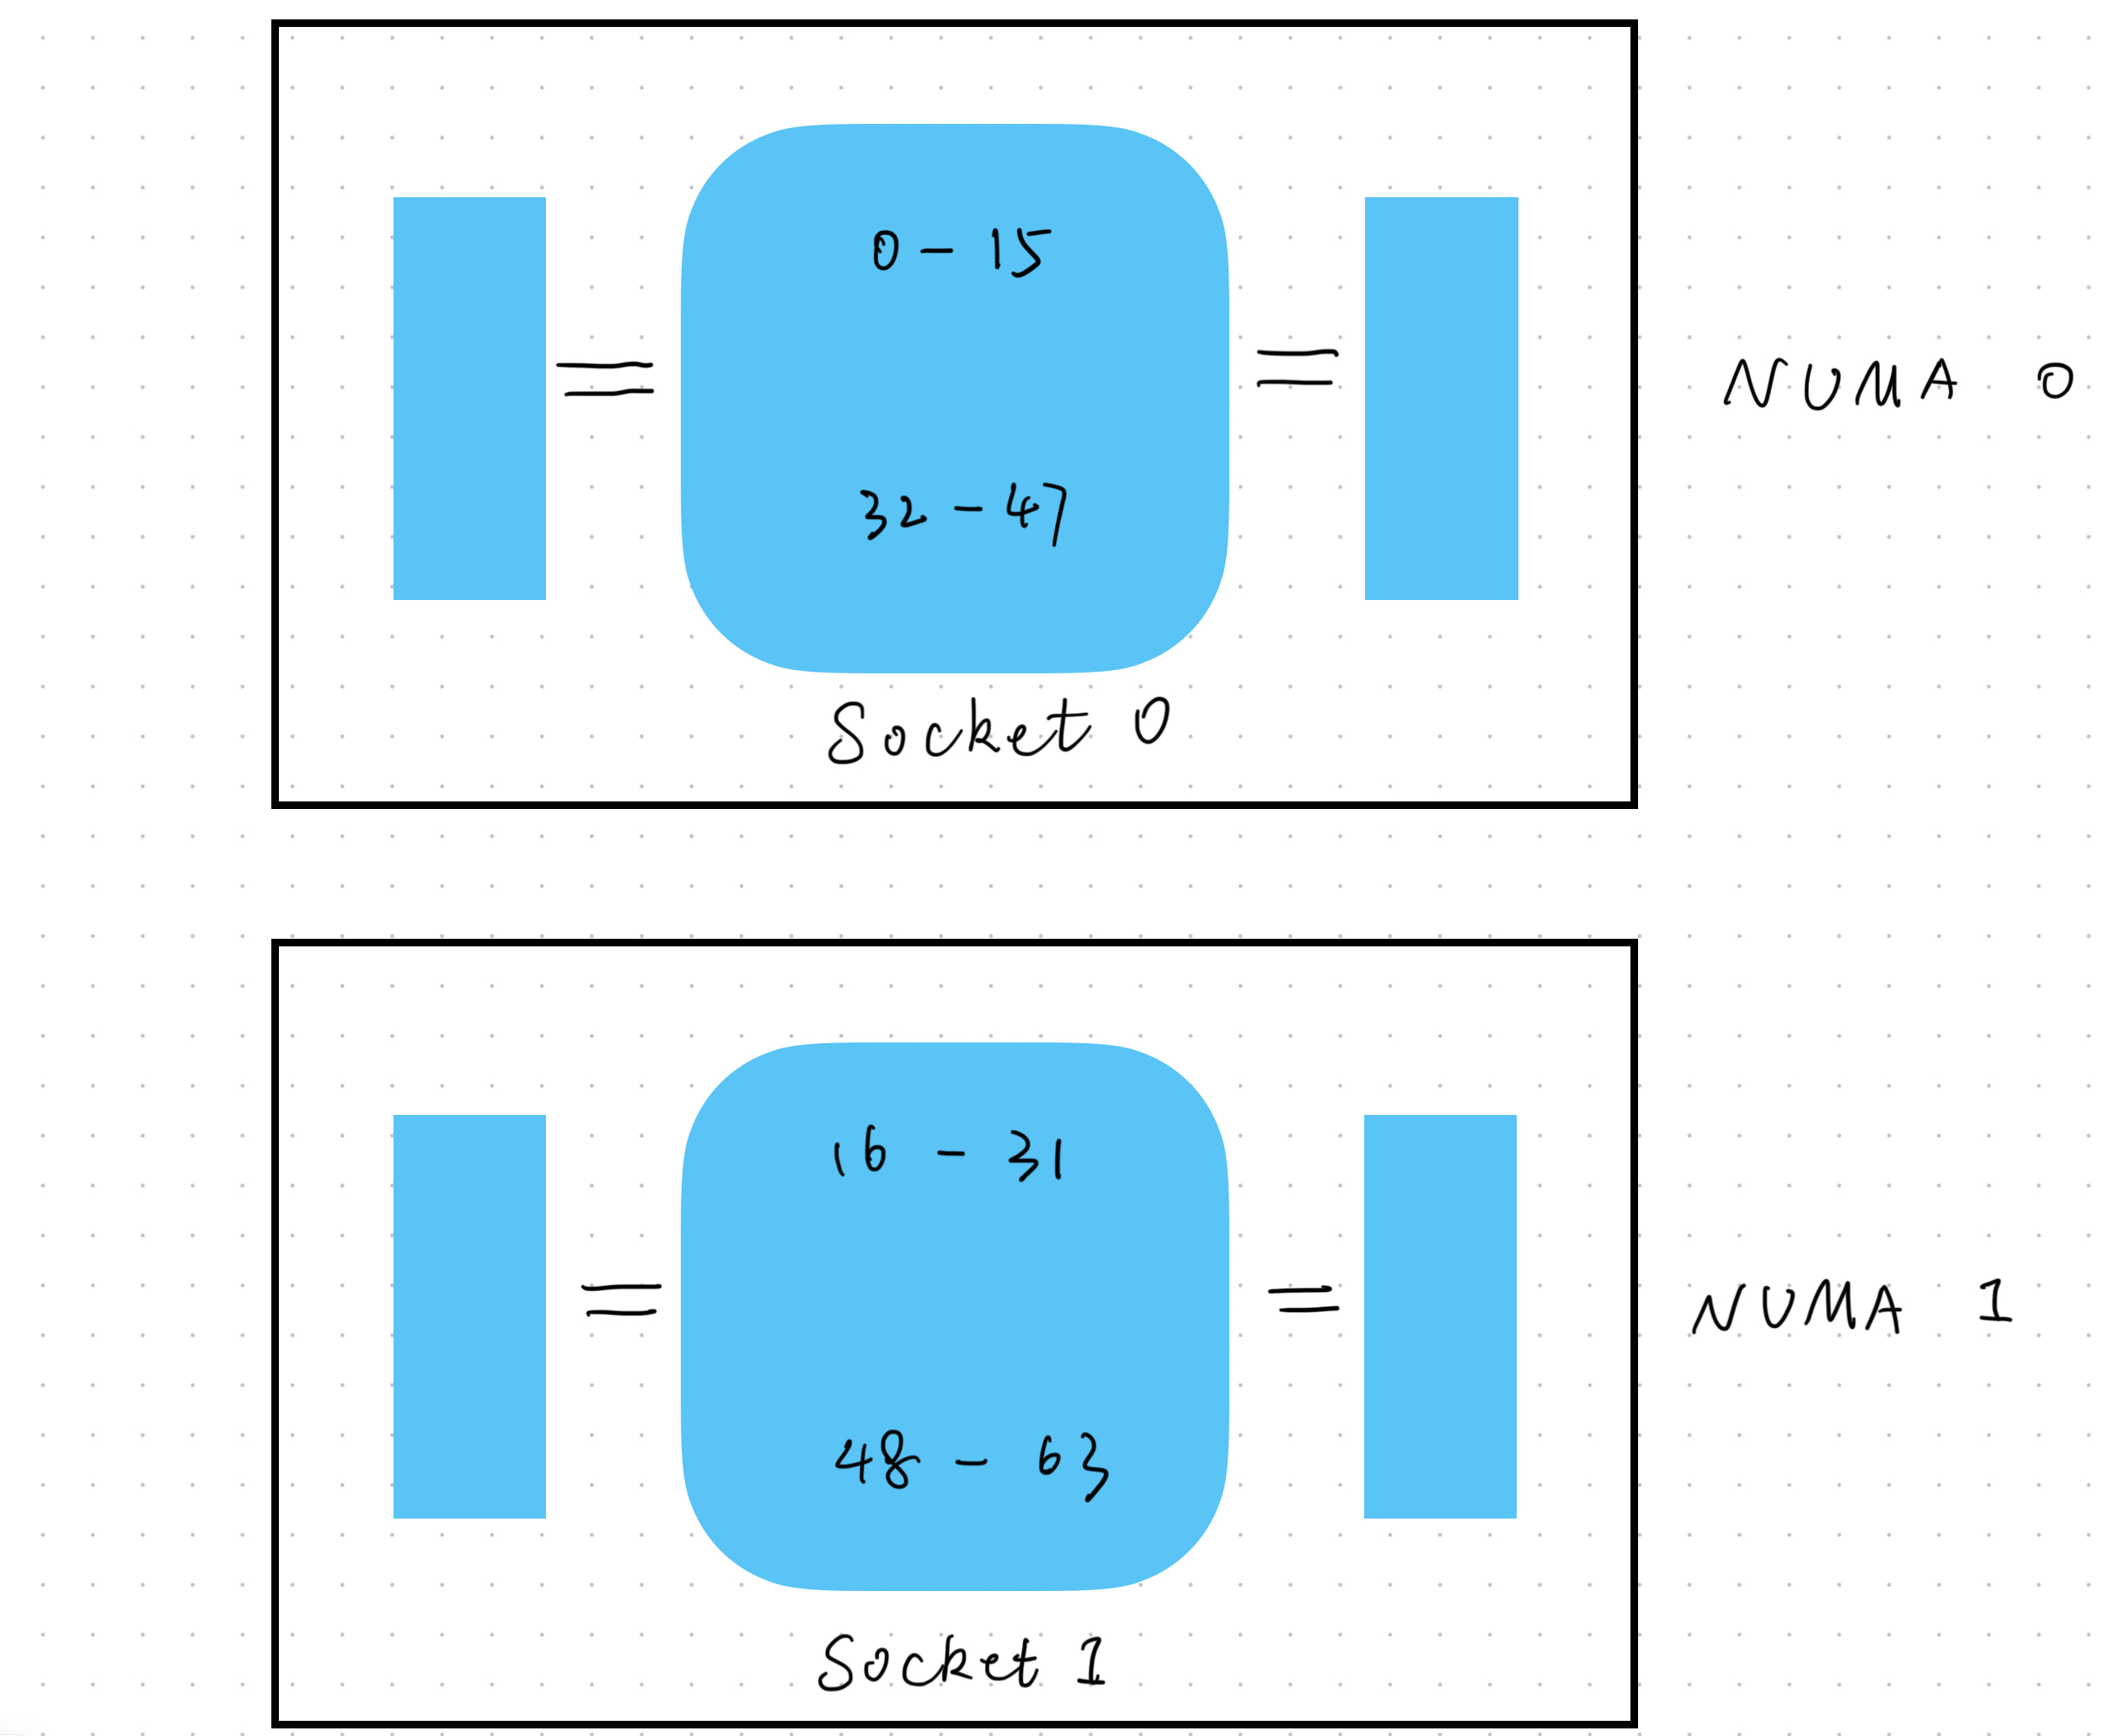
\includegraphics[width=0.5\textwidth]{figure/FIG_Topology_Callan.jpg}
  \caption{NUMA topology of single node on Callan}
  \label{FIG_Topology_Callan}
\end{figure}
Accessing the other NUMA node's memory reduces the bandwidth and also the latency,
though the bandwidth is commonly high enough, the latency can increase by 
$~30\%$ to $~400\%$ \cite{NUMA_Latency_TCD}. 
This latency becomes dangerous when writing shared memory parallel programms.




% In this project, I chose to use various numerical approaches to approximate the solutions.
% It begins with Finite Difference Methods(FDM) and an other method employed by deep neural 
% networks which leverage by their capability as universal function approximators
% \cite{DNN-HORNIK1989359}. 

% The Kormoglov PDEs are series of equations which describe the motions of Brownian Motions
% \cite{SolveKorPDE}.
% In general, 
% let $T \in (0, +\infty)$, $d \in \mathbb{N}$, 
% let $\mu : \mathbb{R}^d \rightarrow \mathbb{R}^d$ 
% and $\sigma: \mathbb{R}^d \rightarrow \mathbb{R}^{d \times d}$ be the Lipschitz continuous fucntions.
% Let $\varphi : \mathbb{R}^d \rightarrow \mathbb{R}$ be a function, 
% and $u$ be a function from Hilbert Space 
% $[0, T] \times \mathbb{R}^d$ to $\mathbb{R}$
% \begin{align*}
%   u : [0, T] \times \mathbb{R}^d & \longrightarrow \mathbb{R} \\
%       (t, x) & \longmapsto u 
% \end{align*}
% with at most polynomially growing partial derivatives.
% The problem is that $u$ satisfied a below system on $D = [0, T] \times \left[a, b \right]^d $ and 
% $a, b \in \mathbb{R}^d$ with $a < b$,
% \begin{align}
%   & \frac{\partial u}{
%     \partial t} 
%   = \frac{1}{2}
%   \text{Trace}_{\mathbb{R}^d}
%   \left[
%     \sigma(x) \sigma^{*}(x)
%     \left(\text{Hess}_x u\right)
%   \right]
%   +
%   \langle 
%     \mu, 
%     \nabla _x u
%   \rangle_{
%     \mathbb{R}^d
%   } \\
%  & u(0, x) = \varphi(x), 
%  \:\:\:\: 
%  x \in \left[a, b \right]^d
%  \\
%  & \left.
%  \left(
%   \frac{\partial u}{\partial \vec{n}}  + \lambda u 
%  \right)
%  \right|_{x \in \varGamma}
%  = g(t, x) 
%  \:\:\:\: 
%  \forall t \in [0, T],\: x \in \mathbb{R}^d
% \end{align}

% The goal is to numerically appriximate the stablized state $u(T, x)$ of the system in the fureture time $T$,
% and in the hypercude space $\left[a, b\right]\in \mathbb{R}^d$ with various boundary conditions $g$.

% Reprompt problem, this work aimed at solving this problem in a bigger picture which requires a more general 
% form. 
% In this project, I consider the parametrized and nonliner PDEs of the general form
% \begin{align}
%   \frac{\partial u}{\partial t}
%   + \mathcal{N} 
%   \left[
%     u; \lambda
%   \right] 
%   = 0
%   \:\:\:\: 
%   t \in \left[0. T\right], x \in D
% \end{align}
% where $\mathcal{N}\left[\cdot; \lambda \right]$ stands for a nonlinear operator parametrized by $\lambda$.
